\documentclass[design, pageheader]{njubachelor}
\usepackage{njusebachelor}

\sid{151250038} %学号
\grade{2015} %年级

\cauthor{刚昭} %学生姓名
\ctitle{基于不完整示例的跨应用自动填表} %题目
\cdepartment{软件学院} %院系
\cspecialization{软件工程} %专业
\cmentor{蒋炎岩}{助理研究员} %指导老师 职称
\ckeywords{数据预处理;程序合成;表格转换} %关键词
\cdate{2019.05.15} %提交日期

\eauthor{Zhao Gang} %UNDERGRADUATE
\etitle{Synthesize Application-Agnostic Spreadsheet Table Transformation Program from Partial Output Example} %THESIS
\edepartment{Software Institute} %DEPARTMENT
\especialization{Software Engineering} %SPECIALIZATION
\ementor{Yanyan Jiang}{Assistant Researcher} %MENTOR MENTORTITLE
\ekeywords{Data Wrangling; Program Synthesis; Table Transformation} %KEY WORDS

\begin{document}

\makectitlepage

\begin{cabstract}
在日常的计算机使用中,用户经常会需要将一种形式的表格转换成另一种形式,而且往往会跨应用。如果用户拥有熟练的编程技能,这类重复性极强的“复制粘贴”工作可以很方便地自动化,但是大部分用户都没有这个条件。在相关的研究工作中,基于示例的程序合成是一个很有前景的方向,这类工作要求用户提供一对完整的输入输出示例,即一个原始形式的表格和一个想要的形式的对应表格,然后就可以根据这对示例自动生成一个程序,使其能将类似形式的输入转换成类似形式的输出,用户之后再遇到类似的任务时,直接运行该程序即可。然而,这类已有工作对用户提供的示例要求较高,用户需要花费一些精力来首先抽象当前任务,这往往要求用户自己认真准备一组示例表,这种做法对用户并不友好,在用户经常需要处理新任务时会给用户额外的思考和操作负担。为此,我利用了一些此类任务中表格的特性,设计了一种新的用于表格转换的程序语言以及配套的自动生成该类程序的算法,只需要用户提供部分当前任务的输出示例,就可以生成可靠的程序。该放松了输入条件的新方法有更广泛的潜在应用,我将描述一个可以将该技术应用到不同领域的技术框架,例如处理 Word 文档里的表格、自动填充网页表单、对爬虫数据进行预处理等。用户在获得想要的程序后,不但可以拿这个程序处理当前的任务,还可以将它保存下来,将来拿它处理任何不同应用、相似需求的任务。

为了检验算法和框架的实际效果,我开发了一个基于 Electron 的跨平台桌面端应用。在需求开发方面,我在蒋炎岩老师的帮助下对计算机系教务员进行了访谈,在确立了一些用例后,独立实现了对 Word 文档内的表格读取和在内嵌的 webview 网页中进行 record-replay 的功能,使其可以完成例如将本地 Word 文档中保存的课程表自动填到教务系统中的任务。另外,该新方法能够处理一些已有工作不能解决的表格转换任务。
\end{cabstract}

\begin{eabstract}
End-users often need to transform tables from one layout form to another, potentially cross-application.
Writing programs can alleviate these repetitive tasks, but many users do not have such a skill.
Program Synthesis by Example is a promising approach which can automatically synthesize a target program using user-provided examples.
Existing techniques ask the user to provide a concise and complete pair of input-output example, but in real world such requirement will take the users' nonnegligible efforts to abstract their current tasks, and thus impose huge overhead if the users' tasks change frequently.
We present a new language of programs for table transformation as well as an algorithm to automatically synthesize such programs by asking the user to only provide a partial output example for the current task.
Our technique is broadly applicable.
We describe a framework to apply such technique to different problem domains such as Word Document and Web Forms.
A user can not only use the synthesized program to perform the current transformation task, but also save the program and use it later to automatically transform other tables with similar layout, from and to different applications. 

To evaluate the practicality of our language, algorithm and framework, we built a desktop application which can take csv or docx files as input and generate csv files or web forms as output.
Our approach can handle cases that previous works cannot, and our user testing with university staff showed that our application can successfully meet end-users' variety of transformation needs.    


\end{eabstract}\nopagebreak

\pagenumbering{Roman}

\maketoc
\newpage

\listoffigures
\listoftables
\newpage

\pagenumbering{arabic}

\section{第一章~引言}

\subsection{项目背景}
填表,是一件所有人都会不断重复做的事。表格类型多种多样,如汇总表,常见的有财务报表,成绩表,实验表;单表,常见的有阶段报告,出差申请。表格涉及的应用也多种多样,以不同格式出现:Word 里的 docx 文件,Excel 里的 xlsx 文件,Web 里的 form 等。由于不同表格形式不同且跨应用,用户经常要在不同表之间复制粘贴,浪费大量时间,也会因为注意力不够集中引发错误\cite{stolee09}。

由于表格自身在空间上结构化的特点,以及不同表格间内容的高度重复性,填表本身是一件可以被高度自动化的工作,而且 Excel 等办公软件也提供编写自定义脚本的功能,用户可以使用 VBA 语言来编写处理表格的程序。然而,需要经常填表的用户,大部分都不是程序员。Excel Help Forum\footnote{Excel论坛程序板块网址:https://www.excelforum.com/excel-programming-vba-macros/}上有大量用户询问如何编程的帖子。

除了文职管理人员需要在办公时填写大量的表,表格转换作为数据预处理的一类操作,在数据分析工作中有重要的地位\cite{kandel11.2}。一项工业界的调查报告指出\footnote{报告详情:https://visit.figure-eight.com/rs/416-ZBE-142/images/CrowdFlower\_DataScienceReport\_2016.pdf},数据分析师工作中 80\% 的时间都在进行收集数据、清理数据等数据预处理工作,将数据转换成分析工具所需要的格式。

当用户需要自动化一个操作任务时,往往心中对操作的结果有一个预期,知道结果该有的形状和内容,只是不知道如何写程序达成该预期。基于示例的程序合成便是一类非常实用的技术,在很多领域都有成功应用\cite{feser15}\cite{smith16}\cite{rolim17},用户只需给定输入输出的样例,这些工作就能自动地为用户生成想要的程序。

交互式、基于示例的程序合成长期以来都是研究表格转换的重点\cite{gulwani15},其主要任务是推理出一个能正确映射用户对表格数据的处理的函数,如发现用户想要使用的正则表达式\cite{raza17}、字符串变换\cite{gulwani11}等。虽然这类任务的确经常困扰没有编程经验的终端用户,但对于不对源数据进行修改的跨表复制粘贴这一类布局转换操作,却一直缺少足够自动化、跨平台、易扩展的自动填充工具。现有的自动填充工具,工业界方面存在大量的只支持 web 的个人信息管理工具,如 RoboForm\footnote{RoboForm 工具官网:https://www.roboform.com/}, Dashlane\footnote{Dashlane 工具官网:https://www.dashlane.com/} 等。学术界也有一些基于单一系统内的数据和上下文特点做自动填充的工作,如跨 web 应用填表工具\cite{wang13}。它们实现复杂,且都不够通用。Office 扩展商店里唯一相关的插件是 Excel-to-Word Document Automation, 但其只支持 Excel 到 Word 表格一对一的整体映射,解决场景过于单一,不能解决批量的不同布局形式的表格之间的转换。通过我们的需求调研,我们确认类似以上的场景真实存在,尚没有足够好的解决方案。

我们的表格是指 Spreadshee Table 而非更结构化的关系型数据表。Spreadsheet Table 的每一行每一列的名称可能没有给出,不同行的单元格的数据类型和语义可能不同。Spreadsheet Table 具有固定的行列数。即使对于一张非矩阵表如 Word 中被部分切割的表格,也可以通过扩充行列的形式对齐后转换成一张矩阵形式的标准 Spreadsheet Table。这种 Spreadsheet Table 的定义相比于关系型数据表能适应于更广泛的跨应用填表的场景,如将 Word 文档中不规整的表填到 Excel 的汇总表。Spreadsheet Table 的应用范围更广,但也同时缺少了一些结构化的信息,带来了程序设计上的挑战。下文中出现的 Table 均指 Spreadsheet Table。

我们发现,用户在遇到重复性强的任务需要自动化的需求时,其实往往能够提供一个实体性质的输出示例,且输出示例中同一列的值往往具有特定语义。根据这个实体示例和源表格的映射图,我们可以利用一种启发式规则来判断出关键索引列,即发生多对一映射现象的特定类型数据。多对一映射指输入表中多个单元格的值与一个且仅一个输出单元格的值相等。为了填充输出表中的其他内容,我们观察到可以通过在关键索引列的单元格上建立游标,通过这些游标的集体移动来逐步填完输出表。表格转换程序只需记录索引列号和游标的移动与映射规则,即可将其它任意类似布局的输入表转换成用户需要的输出表。

基于这样的思路,我们描述了一个新的只需要一个输出实体示例和完整的源数据表就可以自动合成表格转换程序的算法,以及其使用的表格转换程序语言的语法和语义。由于我们算法的特性,用户提供的输出实体示例甚至不需要完整,这一点将在第三章进行描述。

本文中,若无特殊指出,均假设填表时表格的增长方向为纵向增长:列数不变,行数增加。这样的增长方向由于符合关系型数据表的模式,适用范围非常广泛。若用户有横向增长的需求,只需在实现时反转本文中所有提到的方向。

为了说明我们工作的应用前景,我们描述了一个将此技术扩展到不同应用领域的框架,并基于此技术和用户调研,开发了一个跨平台桌面端应用,实现了单表格转换和基于源表格的网页自动填表功能。对用例功能的成功实现验证了我们工作的实用性。

\subsection{国内外研究现状}
\subsubsection{视图变换的程序合成}
用旧表内容填新表可以看作是一个如何进行视图变换的问题。在数据库和程序语言的研究社区中,给定一张原表和其转换形式后的视图,如何推理出一系列变换操作,使其既有和例子的一致性,又不失一般性,是一个经典问题\cite{sarma10}。获得进行变换的程序后,对于待填的格式相近的新表,只要指定其输入数据来源,就可以自动获得其填充后的版本。W. R. Harris等人研究过该问题的 Spreadsheet版\cite{harris11},利用了 Spreadsheet 里的内容相对于数据库关系表有额外的顺序和位置特征,并考虑到电子表格缺少规范的表头信息和依赖关系的缺点,设计了基于坐标映射的操作函数和搜索算法,使其能够处理缺少行列元数据、甚至缺少某些单元格数据的电子表单,同时又能保留原表中的顺序。之后的 Jin 等人的工作则将输出表的格式进一步局限为关系型数据表\cite{jin17},并在程序语言上改用已由 Raman 等人\cite{raman01}定义的表格转换的操作符,这些操作符不但包括用于布局转换的操作符,还包括如 Split, Merge 等修改单元格内容的操作符,因此相较 Harris 的工作可以更精确地完成一些其它种类的表格转换任务。然而,这类工作结果的实际使用有一大局限,这些工作的理想应用场景是用户需要将多张格式统一的旧表转成多张格式统一的新表,因此合理地要求用户给出一个完整的输入输出表的用例,但在用户更多地集中在完成当前任务时,该基于示例的模式并不合适,用户在需要利用软件自动填充单表时,他只会填充了其中一小部分,提供完整的样例需要用户对任务做额外的抽象,引入更多的思考和操作负担。

在对程序的搜索空间的定义上,除了上述的语法制导的逐步构建程序的途径,还有通过软件挖掘的方式从已有的转换脚本中搜索满足需要的方法,如 He 等人\cite{he18} 的工作要求用户指定输入列以及给出部分输出用例,之后从 Github, Stack Overflow 的代码中找到一个能将输入列的格式正确转换成符合输出用例格式的函数。他们的工作主要处理的是某类数据需要统一格式的场景,而非布局样式的转换。

除了这类让用户直接提供输入输出样例的程序合成范式,另一类和填表潜在相关的是S. Gulwani 提出的基于自然语言描述的程序合成\cite{gulwani14},对常见的用户对任务的表述,如选择行列、filter类型操作、reduce类型操作等建立领域特定语言,再将用户描述直接翻译成所需要的程序。考虑到该方法对用户表述问题的特殊要求,为了软件的易用性,我们不打算采用这类方法。

\subsubsection{交互式数据处理}
人机交互的研究社区中,有大量工作旨在帮助终端用户即没有编程技能的用户完成包含数据抽取、数据清理、数据转换等一系列的工作,从而使他们将原始数据变换为自己做分析所需要的形式。 Wrangler\cite{kandel11} 是一个代表性的例子,并拥有后续的商业版本 Trifacta。Wrangler 利用大量的预设操作和推荐算法,对用户在数据表格上的操作意图进行预测,自动进行批量的选择、删除、行列变换、聚类等操作,从而达到缩短完成任务所需时间的目的。然而,此类工作的有效性是建立在用户需要一步步指定转换操作之上的,其面对的是有数据处理经验的数据分析师。为了精确描述自己想要的转换,用户要从源数据表格出发,从给定的操作列表中逐步选择自己想要的操作,直到完成自己想要的转换。这种非声明式的途径对没有技术背景的用户很不友好,需要的用户操作也很多。我们通过用户调查发现,当用户有一个表格转换的任务需求时,往往心中有一个明确的输出示例,但却很难程序化地描述这种转换操作。

\subsubsection{更好的复制粘贴}
人机交互社区里有很多对复制粘贴进行改进的工作,其中和我们最相似的一个是Citrine。Citrine \cite{stylos04} 替换了复制粘贴步骤里的后台剪贴板部分,不影响复制和粘贴的操作,具有很高的易用性和可扩展性。它拥有自己的粘贴板格式,靠附加的前端的 parser 和后端的 generator 在不同应用的不同格式数据间复制粘贴。用户复制一段 parser 能识别的数据时,其数据可能是结构化的有标记的数据,也可能是纯文本。parser 会依据内置的模式检查,为纯文本的内容项打上例如联系方式或日程项的标签,然后将其转换为自己统一的结构化的粘贴板中间格式,之后用户再在需要粘贴的位置进行粘贴操作,generator 根据粘贴位置的结构化信息和其应用类型,在相应的位置填充对应的数据。Citrine 不能解决复制粘贴这一操作本身耗时、易出错的根本问题。

\subsection{论文的主要工作和组织结构}

第一章:概述和前言部分,介绍了项目背景、当前表格程序合成与数据处理的研究现状,并描述了该论文的主要工作。

第二章:主要介绍了程序合成技术、应用开发过程中使用到的基于浏览器端的录制重放技术。

第三章:描述了用于表格转换的程序语言、自动根据示例合成该类程序的算法,以及它们的具体实现。

第四章:描述了将算法实现应用到不同领域的技术框架,并结合需求分析手段,描述了一个特定的自动填表应用的具体功能性和非功能性需求。

第五章:描述了该自动填表应用的详细设计与实现。

第六章:总结论文的工作和创新点,讨论其中的不足和未来可能的扩展方向。

\section{第二章~自动填表应用技术概述}

\subsection{语法制导的基于示例的程序合成}
程序合成的定义为:寻找一个功能性函数 {\itshape f} 使得一个用于检验 {\itshape f} 正确性的逻辑公式$\varphi$的值恒为真。该逻辑公式代表了该程序的需求规约。\cite{alur13}大部分程序合成的算法可以看作在解决一个搜索问题(其它的可能算法包括程序转换,从现有的已经正确的程序出发,一步步转换成满足某些特定指标的语义等价的目标程序,常用于性能优化\cite{schkufza16}):在程序语言确定之后,直接从所有可能的程序中搜索出一个符合语法的且满足需求规约的程序。语言可以是通用的编程语言如 Java,但如果使用此类通用语言进行搜索,会容易出现搜索空间过大、过拟合等问题。使用自定义的领域特定语言 DSL (Domain Specific Language),能够通过限制搜索空间来显著加快搜索速度,提高程序鲁棒性,也能使生成的程序更容易理解。\cite{alur13} 此类途径被称为语法制导的程序合成。此类工作需要定义特定的表达式和上下文无关文法,目标程序即由一组表达式组成。这些表达式可以来源自现有的形式化理论,例如线性整数运算 LIA (Linear Integer Arithmetic) 中定义的 int 和 boolean 类型值, boolean connectives ($\wedge$, $\neg$), addition(+), comparison($\leq$, $\geq$) 和 conditionals ({\itshape ITE})。假如需要合成一个返回 x 和 y 中最大值的程序,其可能的语法定义为:

{\itshape T:= x | y | 0 | 1  | ITE(C, T, T)}

{\itshape C:= (T$\leq$T) | (T$\geq$T) | $\neg$C | (C$\wedge$C)}

其可能的程序规约的逻辑公式为:

{\itshape (f(x,y) $\geq$ x) $\wedge$ (f(x,y) $\geq$ y) }

如下程序即是一个满足该语法和规约的正确的程序:

{\itshape f(x,y) = ITE(x $\leq$ y, y, x)}

给定一个特定的问题场景,已有的形式化理论很可能没有一个能高效适用的,此时可以通过定义各种符号具体的语义来自定义一个形式化理论。如本工作就使用了自定义的语义。在此类工作中,用于检验正确性的逻辑公式通常为基于其特定使用的形式化理论的一阶谓词逻辑。

对于用于检验程序正确性的需求规约,可以由书写合成算法的人形式化地直接给出,此类方法称为基于约束的程序合成;也可以由一组输入输出示例表示,生成的程序在接受输入示例后能生成预期的输出即视为正确,此类方法称为基于示例的程序合成。

实际的搜索过程是一个 NP 问题,为了高效地进行搜索,可以利用现有的 SMT (Satisfiability Modulo Theories) 求解器,尤其是当使用的形式化理论为已有的理论时。但如果问题的搜索空间不大,应用场景没有特殊的性能要求,那么暴力枚举搜索也是可以接受的。

\subsection{录制重放技术}
为了使应用支持自动完成重复的网页填表任务,结合我们让用户输入部分输出示例的前提,我们需要能够记录用户在这一次示例填表过程中对什么页面元素填了什么值,这样我们的应用就能对其它待填原始数据执行相同的搬运动作,完成自动填表的任务。

录制重放是一个在软件工程领域被广泛讨论的话题,开发者可以通过一些具体的 tracing 方式,记录下用户与其应用的交互序列或是应用底层的行为,使这一段软件的行为可以在其它机器、其它时间复现。这类技术可用于调试用户遇到的 bug \cite{burg13}、在线检测错误\cite{ronsse99}等。在本份工作中,我们利用录制重放技术来重复执行用户对应用的一系列操作,以达到减轻用户负担的目的。

\subsection{Electron桌面端应用框架}
Electron 是一个知名的支持 Web 开发技术栈的跨平台桌面端应用开发框架,当下许多流行的软件如 Visual Studio Code\footnote{VS Code 的 GitHub 项目页:https://github.com/microsoft/vscode}, Slack\footnote{Slack 关于使用 Electron 的技术博客:https://slack.engineering/tagged/electron} 都是基于 Electron 开发的。我们的项目选择它的主要原因是开发人员较熟悉该应用开发框架,以及使用桌面办公软件如 Microsoft Office 的用户至少跨越 Windows 和 Mac 平台的跨平台需求。每个 Electron 应用界面的实质都是网页,由 HTML, CSS, JavaScript 组成。Electron 使用自己封装的 Chromium 浏览器渲染这些界面,利用 Node.js 来完成与本地操作系统交互的部分。

如果选择开发一个 Web 应用,也可以满足跨平台的需求,但我们考虑到表格转换这一通用的功能可能需要在封闭的内网或无网环境中使用,所以最终还是选择了桌面端。

\subsection{本章小结}

本章介绍了本工作的核心技术程序合成相关的背景知识,并补充介绍了应用开发使用到的录制重放技术、Electron 桌面端应用框架。另外,本章描述了使用这些技术的动机,讨论了使用它们的合理性。

\section{第三章~表格转换的程序语言及其基于不完整示例的合成算法}
\subsection{语言和算法描述}
在一张 Table 中,每个单元格的位置都可以用行列对表示,如(1, 2)表示第1行第2列。本文中的行列遵循 Spreadsheet 应用的传统,从1开始而非从0开始编号。一个映射序列包含了一组有序的映射关系,每个映射关系是一个有序坐标对,两个坐标分别属于不同 Table,坐标对的第一个元素称为输入坐标,第二个元素称为输出坐标。程序 MapProg 的语法定义如图\ref{fig:map_prog}所示。 接下来我们从操作的角度描述操作符的语义。

\begin{ttmath}
$\bullet \mathtt{MTOTRANS(IndexProg,{TrailProg_{1},...,TrailProg_{n}})}$: 作用于表格$T_{I}$时,生成 $IndexProg$ 和所有 ${TrailProg_{i}}$ 在该表格上作用后返回的映射序列列表的并集(ZIP),按顺序将该并集映射序列列表中每个映射关系的对应$T_{I}$单元格内容填到输出单元格中。

$\bullet NORMTRANS(MAP)$: 作用于表格$T_{I}$时,将首先按照$MAP$和$T_{I}$的内容填充输出表,之后执行以下循环:将$MAP$中的所有输入坐标的行号加$MAP\_INPUT\_MAX\_ROW$,所有输出坐标的行号加$MAP\_OUTPUT\_MAX\_ROW$,再按该新$MAP$填充。当$MAP$的输入坐标在$T_{I}$中的值全为空时,循环结束,该操作结束。

$\bullet INDEXMAPPING(INDEXCOL, OUTCOORD, STARTROW)$: 作用于表格$T_{I}$时,将$T_{I}$中$INDEXCOL$列的单元格从第$STARTROW$行开始按单元格内容是否相同进行分组,之后按组内单元格的最小行号对组进行增序排列,组内也按行号增序排列,得到一个坐标组序列。以这些坐标组序列中的坐标为输入坐标,$OUTCOORD$为输出坐标,遵循相同的组内和组间顺序建立一个映射序列列表。返回该映射序列列表。

$\bullet TRAILMAPPING(IndexProg, Movement)$: 作用于表格$T_{I}$时,对$IndexProg$作用在$T_{I}$上生成的一组映射序列中的每一个映射序列使用$Movement$获得变换后的映射序列。返回变换后的新的映射序列列表。

$\bullet ROWOUT(MOVE\_X, MOVE\_Y, OUTROW, FIRST\_OUT\_INDEX)$: 作用于映射序列$MAP$时,将$MAP$中所有输入坐标的行号加$MOVE\_X$,列号加$MOVE\_Y$;将所有输出坐标改成行号均为$OUTROW$,列号从$FIRST\_OUT\_INDEX$开始每次递增一的坐标序列。返回变换后生成的新映射序列。
\end{ttmath}

\begin{figure}[!htbp]
    \begin{ttmath}
    \begin{align*} 
MapProg := & MTOProg \mid NormProg \\
MTOProg := & {\textbf {MTOTRANS}}({IndexProg, \{TrailProg_{1}, ..., TrailProg_{n}\}}) \\
NormProg := & {\textbf {NORMTRANS(MAP)}} \\
IndexProg := & \textbf {INDEXMAPPING}(\textbf{INDEXCOL}, \textbf{OUTCOORD}, \textbf{STARTROW}) \\
TrailProg := & {\textbf {TRAILMAPPING}}(IndexProg, Movement) \\
Movement := & \textbf {ROWOUT}(\textbf{MOVE\_X}, \textbf{MOVE\_Y}, \textbf{FIRST\_OUT\_INDEX}, \textbf{OUTROW}) \\ &\mid \textbf{COLOUT}(\textbf{MOVE\_X}, \textbf{MOVE\_Y}, \textbf{FIRST\_OUT\_INDEX}, \textbf{OUTCOL})
    \end{align*}
\end{ttmath}
    \caption{MapProg语法定义}
    \label{fig:map_prog} 
\end{figure}

合成一个 MapProg 的合成算法如图 \ref{fig:map_prog_inference} 所示。

$\bullet \mathtt{GetMap}$会按输出表的 row major order 获得一个映射序列,使得映射序列中的每个映射关系都是一个值相等的关系,且每一个在源表中有相同值的输出表单元格的坐标一定都在该映射序列中。表的 row major order 是指逐行扫描的顺序,即从第1行开始,由该行的第1列到最后一列,然后开始下一行,以此类推。当出现多对一映射时,按输入表的 row major order 顺序保存该多对一映射中的所有映射关系对。

$\bullet \mathtt{SelectionRules}$是一个经验性地用来判断映射序列中的每组多对一映射是否真的是索引列的映射的一阶谓词公式,作用于一个任意的映射序列,可由领域专家进行自定义,本工作的实现中使用的谓词为:

$\mathtt{UniqueInCol(ManyToOneMap, CandidateMTOMaps)}$ 如果 $\mathtt{ManyToOneMap}$ 中的输入坐标在同一列,且该列号在输入表中仅出现在该$\mathtt{CandidateMTOMap}$,则返回真

之所以使用这个谓词,是因为我们通过经验发现,特定索引列普遍存在,且用户提供的单输出实体示例通常只包含一个有索引意义的单元格。

$\bullet \mathtt{ExistsManyToOne(Map, SelectionRules)}$会将$\mathtt{Map}$中出现多对一映射的映射关系按输出单元格进行分组,并检验$\mathtt{SelectionRules}$在每组上的取值是否为真,如有一组为真,则返回真。

$\bullet \mathtt{ExtractMTO}$返回$\mathtt{ExistsManyToOne}$找到的一个映射序列。

$\bullet \mathtt{GetAllowedMovements(T_{I}, MTOMap)}$返回一个整数对集合,该集合满足如下性质:$\mathtt{MTOMap}$中任何一个输入坐标在加上集合中的任何一个整数对后,坐标总为正,且列数不超过$T_{I}$的总列数$\mathtt{ColNum}$,行数不超过$T_{I}$的总行数$\mathtt{RowNum}$。函数的详细操作为:定义$\mathtt{SmallestCol}$ 为 $\mathtt{MTOMap}$的输入坐标中的最小行号,$\mathtt{LargestCol}$ 为 $\mathtt{MTOMap}$的输入坐标中的最大行号,$\mathtt{SmalletsRow}$和$\mathtt{LargetstRow}$同理,则对于每一个范围在$\mathtt{(-SmallestCol + 1, (ColNum - LargestCol) - 1)}$的整数值x,和每一个范围在$\mathtt{(-SmallestRow + 1, (RowNum - LargestRow) - 1)}$的整数值y,将数对(x, y)放入结果集合中,最后返回结果集合。

$\bullet \mathtt{GetFirstIndexInRow(MTOMap, \Delta X, \Delta Y, T_{I}, ROW, T_{O})}$返回$\mathtt{T_{O}}$中第$\mathtt{ROW}$行的与$\mathtt{MTOMap}$中第一个映射关系的输入值相等的单元格的列号,若无则返回1。

$\bullet \mathtt{IsConsistent(Prog, T_{I}, ExampleMap)}$取$\mathtt{Prog}$作用在$\mathtt{T_{I}}$上获得的映射序列列表中的第一个映射序列$\mathtt{FirstMap}$,若$\mathtt{ExampleMap}$是$\mathtt{FirstMap}$的子集,则返回真。


\SetKwInput{KwInput}{Input} 
\SetKwInput{KwOutput}{Output} 
\begin{figure}[!htbp]
    \begin{ttmath}
    \begin{algorithm*}[H]
        \setstretch{0.78}
    \caption{Synthesize MapProg by example}
    \SetAlgoLined
    \KwInput{source table T$_{I}$, output example table T$_{O}$}
    \KwOutput{ MapProg, or \textbf{error} if no consistent MTOProg is found }
        \tcc{Step 1): detect if there is many-to-one mapping}
        $CurrentMap \leftarrow GetMap(T_{I}, T_{O})$;\\
        \If{ExistsManyToOne(CurrentMap, SelectionRules)}
        {
            \tcc{Step 2a): construct IndexProg}
            $MTOMap \leftarrow ExtractMTO(CurrentMap, SelectionRules)$;\\
            $IndexProg \leftarrow INDEXMAPPING(InCol(MTOMap), OUTCOORD(MTOMap), FirstRow(MTOMap))$;\\
            \tcc{Step 3a): search TrailProg}
            $TrailProgList \leftarrow \emptyset$;\\
            \For{$\Delta X, \Delta Y \in GetAllowedMovements(T_{I}, MTOMap)$}
            {
                $Found \leftarrow false$;\\
                \For{$Col \in GetColNums(T_{0})$}
                {
                    $FirstIndex \leftarrow GetFirstIndexInCol(MTOMap, \Delta X, \Delta Y, T_{I}, Col, T_{O})$;\\
                    $Movement \leftarrow COLOUT(\Delta X, \Delta Y, Col, FirstIndex)$;\\
                    $TrailProg \leftarrow TRAILMAPPING(IndexProg, Movement)$;\\
                    $TrailMap \leftarrow Movement(MTOMap)$;\\
                    \If{$(IsConsistent(TrailProg, T_{I}, TrailMap))$}
                    {
                        $TrailProgList \leftarrow TrailProgList \cup \{TrailProg\}$;\\
                    }
                }
                \If{$Found$}
                {
                    $break$;\\
                }
                \For{$Row \in GetRowNums(T_{0})$}
                {
                    $FirstIndex \leftarrow GetFirstIndexInRow(MTOMap, \Delta X, \Delta Y, T_{I}, Row, T_{O})$;\\
                    $Movement \leftarrow ROWOUT(\Delta X, \Delta Y, Row, FirstIndex)$;\\
                    $TrailProg \leftarrow TRAILMAPPING(IndexProg, Movement)$;\\
                    $TrailMap \leftarrow Movement(MTOMap)$;\\
                    \If{$(IsConsistent(TrailProg, T_{I}, TrailMap))$}
                    {
                        $TrailProgList \leftarrow TrailProgList \cup \{TrailProg\}$;\\
                    }
                }               
            }
            \tcc{Step 4a): construct MTOProg}
            $MTOProg \leftarrow MTOTRANS(IndexProg, TrailProgList)$;\\
            \If{$(IsConsistent(MTOProg, T_{I}, CurrentMap))$}
            {
                \Return {MTOProg};\\
            }
            \Else {
                \Return \textbf{error};\\
            }             
        }
        \Else
        {
            \tcc{Step 2b): construct NormProg}
            \Return {NORMTRANS(CurrentMap)};\\
        }
    \end{algorithm*}
    \end{ttmath}
    \caption{MapProg合成算法}
    \label{fig:map_prog_inference} 
\end{figure}

\subsection{合成示例}


为了将表 \ref{table:example_source}
\begin{table}[!htbp]
    \centering   
    \begin{tabular}{|l|l|l|}
    \hline
    部门 & 项目 & 会议日期  \\ \hline
    销售部门  & 新一代通讯设备 & 4.15      \\ \hline
    设计部门   & 新一代通讯设备 & 4.16   \\ \hline
    研发部门  & 新一代通讯设备 & 4.17 \\ \hline
    设计部门  & 电信基建    & 4.20     \\ \hline
    研发部门   & 电信基建    & 4.20    \\ \hline
    \end{tabular}
    \caption{合成示例源表}
    \label{table:example_source}
\end{table}
转换为表 \ref{table:example_target}
\begin{table}[!htbp] 
    \centering   
    \begin{tabular}{|l|l|}
    \hline
     & 新一代通讯设备 \\ \hline
    销售部门   & 4.15      \\ \hline
    设计部门   & 4.16   \\ \hline
    研发部门   & 4.17 \\ \hline
    & 电信基建 \\ \hline
    设计部门   & 4.20     \\ \hline
    研发部门   & 4.20    \\ \hline
    \end{tabular}
    \caption{合成示例目标表}
    \label{table:example_target}
\end{table},可以注意到项目名称是分割重复性任务的依据。用户会为该源表提供如表 \ref{table:example_target_example}
\begin{table}[!htbp] 
    \centering   
    \begin{tabular}{|l|l|}
    \hline
     & 新一代通讯设备 \\ \hline
    销售部门   & 4.15      \\ \hline
    设计部门   & 4.16   \\ \hline
    研发部门   & 4.17 \\ \hline
    \end{tabular}
    \caption{合成示例用户输入}
    \label{table:example_target_example}
\end{table}所示的输出示例。我们假设使用的 SelectionRules 为检查出现多对一映射的源内容是否在同一列,以及该列是否仅有一组多对一映射,如果都是,则返回索引列号。合成算法会首先调用 GetMap 函数,得到映射序列为
\[ 
\left \{
  \begin{tabular}{ccc}
  ((2, 2), (1, 2)), & ((3, 2), (1, 2)), & ((4, 2), (1, 2)), \\
  ((2, 1), (2, 1)), & ((1, 3), (2, 2)), & ((3, 1), (3, 1)), \\
  ((5, 1), (3, 1)), & ((3, 3), (3, 2)), & ((4, 1), (4, 1)), \\
  ((6, 1), (4, 1)), & ((4, 3), (4, 2))
  \end{tabular}
\right \}
\]
其满足 SelectionRules 的 MTOMap 为
\[ 
\left \{
  \begin{tabular}{ccc}
  ((2, 2), (1, 2)), & ((3, 2), (1, 2)), & ((4, 2), (1, 2)) \\
  \end{tabular}
\right \}
\]
即源表第二列为索引列,索引列中不同的值对应每个输出实体的 (1, 2) 位置,索引列的开始行号为2。至此,IndexProg 可以构建完成。
\begin{ttmath}
\begin{nscenter}
$IndexProg = INDEXMAPPING(2, (1, 2), 2)$\\
\end{nscenter}
\end{ttmath}
接下来,程序开始搜索符合要求的所有 TrailProg。最终获得的 TrailProg 为
\begin{ttmath}
\begin{nscenter}
$TrailProg_{1} = TRAILMAPPING(IndexProg, COLOUT(1, 0, -1, 2))$\\
$TrailProg_{2} = TRAILMAPPING(IndexProg, COLOUT(2, 0, 1, 2))$\\
\[\mathtt{TrailProgList}= 
\left \{
  \begin{tabular}{c}
  $TrailProg_{1}$, \\
  $TrailProg_{2}$
  \end{tabular}
\right \}
\]
\end{nscenter}
\end{ttmath}
检验易得,使用由 IndexProg 和该 TrailProgList 组成的程序对表 \ref{table:example_source} 输出的结果与表 \ref{table:example_target_example} 一致,故最终合成的程序为
\begin{ttmath}
\begin{nscenter}
$MapProg = MTOTRANS(IndexProg, TrailProgList)$ \\
\end{nscenter}
\end{ttmath}
该程序在输入为表 \ref{table:example_source} 时的输出正是表 \ref{table:example_target} ,是正确的用户需要的程序。

对于该填表任务,如果用户给定了如表 \ref{table:example_target_partial_example} 的输出示例,则由于其已经提供了关键的索引信息以及我们对 consistent 较为宽松的定义,仍然会获得相同的 \begin{ttmath}$MapProg$\end{ttmath}。我们认为这样的结果具有很强的实用价值,因为在用户实际使用时,会自然希望提供的示例越短越好,可能会认为表 \ref{table:example_target_partial_example} 的示例已经足够完整。尤其是当源表中每个实体的对应行或列有很多,例如有数十个部门时,我们的方法可以显著减少用户的操作量。
\begin{table}[!htbp] 
    \centering   
    \begin{tabular}{|l|l|}
    \hline
     & 新一代通讯设备 \\ \hline
    销售部门   & 4.15      \\ \hline
    设计部门   & 4.16   \\ \hline
    \end{tabular}
    \caption{一个不完整的输出实体示例}
    \label{table:example_target_partial_example}
\end{table}

\subsection{本章小结}
本章描述了本工作的核心贡献:一种新的表格转换程序语言和其基于部分示例的合成算法。本章以一个具体的表格转换任务为例展示了算法的机制,并解释了为什么我们的方法可以允许用户只提供一个不完整的输出示例、讨论了该特性带来的优点。

\section{第四章~自动填表应用框架与需求工程}
\subsection{应用框架}
很多重复性强的计算机操作任务都可以抽象为填表任务,我们接下来将说明,开发者只需要利用我们提供的一个表格定义和一组表格生成接口,就可以很容易地为不同的具体应用编写扩展,实现跨应用自动填表的功能。该框架的类图如图 \ref{fig:uml} 所示,我们的工作提供了 $\mathtt{Core}$ 的实现,其中$\mathtt{Transformer}$是第三章所述的$\mathtt{MapProg}$的具体实现类,$\mathtt{TransformerSynthesizer}$是第三章所述合成算法的具体实现类,$\mathtt{Table}$封装了一个可以按行列号数据结构。框架通过以下一组接口来支持不同应用的填表需求:

$\bullet \mathtt{getOutputUnitSeq()}$: 返回一个$\mathtt{Table}$序列,序列的顺序对应$\mathtt{MapProg}$ 生成的映射序列的顺序,其中每个 $\mathtt{Table}$ 在对应映射序列的每个输出坐标上的值都为其输入表格中输入坐标的值,$\mathtt{Table}$上其它坐标的值为空值。 

$\bullet \mathtt{getOutputTable()}$: 返回$\mathtt{Table}$类型的完整的输出表,是$\mathtt{MapProg}$的所有映射序列映射完成后的结果。

$\bullet \mathtt{getMap()}$: 返回一个完整的由源表到输出表的映射序列。

如果开发者希望支持用户将 Word 文档里的表格内容填到某订票网站上,则可以实现一个读取 docx 文件内容、将其转换为$\mathtt{Table}$格式的 $\mathtt{InputUtil}$,以及一个可将$\mathtt{Table}$内容填到该指定订票网站的$\mathtt{OutputUtil}$。如果开发者还希望支持使用 Excel 电子表格填充相同订票网站,则只需再实现一个读取 Excel 电子表格格式的$\mathtt{InputUtil}$即可。这种前后端分离的模式使开发者为不同应用所需开发扩展的数量为加法而非乘法。本文中的自动填表应用项目就是基于该框架开发的。\\
\begin{figure}
    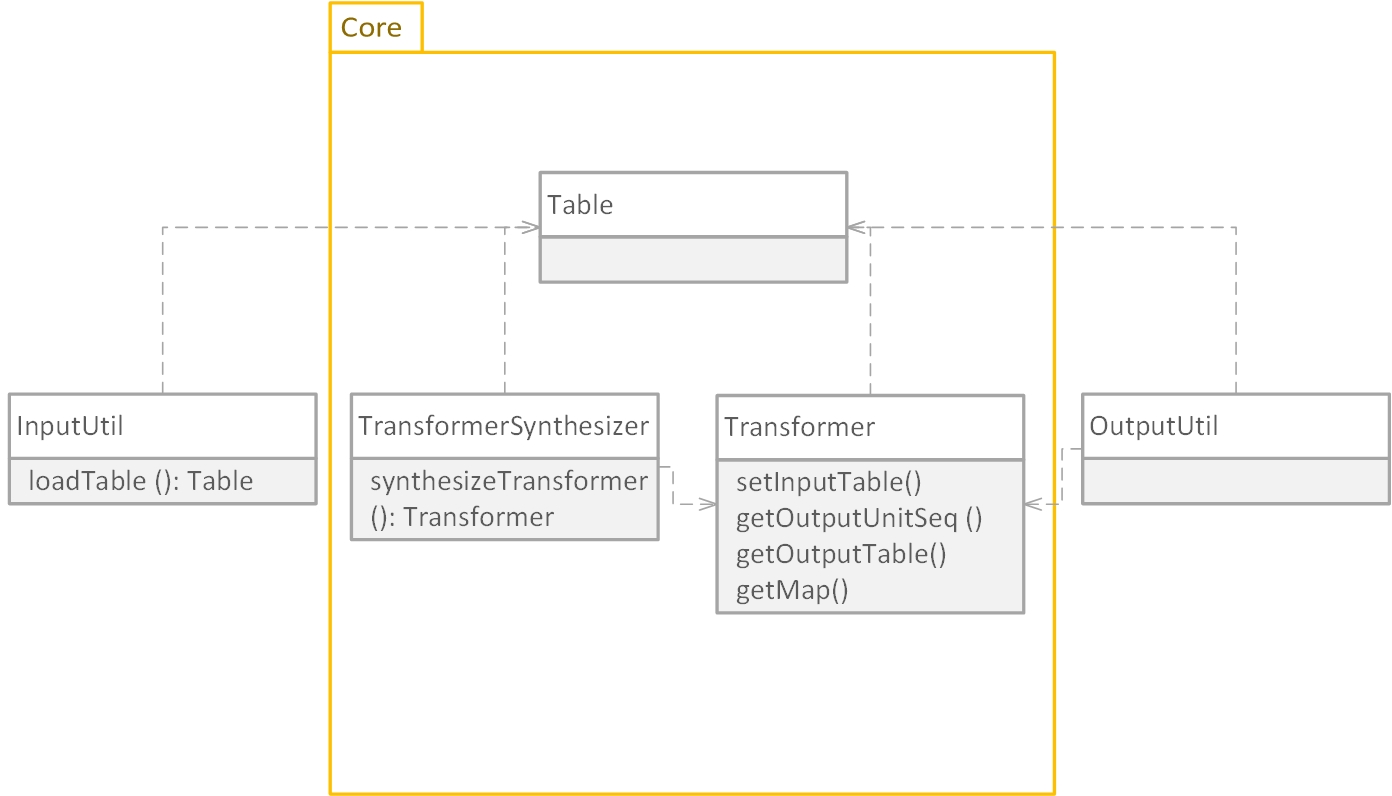
\includegraphics[width=15cm,keepaspectratio]{figures/UML.jpg}
    \caption{自动填表应用框架类图}
    \label{fig:uml}
\end{figure}
\subsection{需求获取}
我们计划开发一个帮助文职人员解决重复性极强的填表问题的项目。为了获得高质量的正式的需求,我们决定寻找有代表性的真实用户进行面谈。

我们找到了一位大学教务员。教务员这一类用户群体相当庞大,所有国内本、专科学校的院系都有独立的教务员。他们经常要和电子表格打交道,且大多没有编程相关的技术经验。他们在上岗前需要专门接受基础级别的 Office 类软件的培训,主要工作例如成绩汇总、排课选课管理、毕业学分统计等都会涉及不同电子表格之间数据的转换。教务员的这些工作在其它管理部门或机构中也有很多相似的对应,如财务报表、档案管理等。因此,教务员是我们系统的理想用户之一,而且由于不涉及商业系统机密,也适合作为我们面谈的对象。

我们计划通过该面谈,回答以下目标问题:

$\bullet${\itshape 问题1. 教务员办公时会在哪些软件上进行填表的操作?}

$\bullet${\itshape 问题2. 教务员有哪些重复程度高的填表操作?是否会跨应用?}

$\bullet${\itshape 问题3. 数据表的来源有哪些?这些表有哪些统一的特征?}

$\bullet${\itshape 问题4. 教务员能够提供的输出示例是否具有完整的实体性?}

$\bullet${\itshape 问题5. 教务员可能出于什么原因放弃使用我们的填表应用?}

我们选择了一个教务员的空闲时间,在其工位上与之面谈,以方便她向我们演示具体的操作场景。结合教务员的非技术职业背景和实地演示的条件,我们选择将面谈设计成开放式面谈,以方便我们在演示过程中引导教务员,发掘她主观上没有意识到的需求。在面谈开始之前,为了提高教务员参与的积极度,我们首先解释了我们应用的可能形式,说服她我们的应用能够为教务员的日常工作提供的巨大便利。

在我们发现教务员已经不再描述新需求时,我们就结束了面谈,整个面谈持续了约1个小时。我们对面谈的内容进行总结,得出目标问题的讨论。

{\bfseries 问题1.} 目前,教务员填表会且只会用到 Microsoft Word, Microsoft Excel, 以及基于 Web 的教务系统。教务系统内只提供了相关数据的下载接口,没有提供数据处理的辅助功能如数据清洗、布局转换等。

{\bfseries 问题2.} 在面谈中,我们一共发现了四件适合自动化的高重复性工作。一是为当前学期课程创建班级。在当前系统中,教务员需要以一张保存在 Word 文档中的课程计划表为源数据,在教务系统中通过选择课程名、填写班级名称、选择上课校区、填写学分数等一系列填写网页表单的操作来完成一个班级的创建,而这些内容全部在 Word 文档的源表中有直接对应,教务员实际做的就是反复的复制粘贴操作。二是二维透视表的创建,如教务员希望将表 \ref{table:regular_scoresheet} 所示的表转成表 \ref{table:pivot_scoresheet} 所示的表。虽然 Excel 软件自带创建透视表的功能,也实际支持创建二维透视表,但我们发现教务员并不了解二维透视表的概念,虽然她拥有透视表的使用基础。三是将多张 excel 单表的内容简单复制粘贴到一起,形成汇总表。四是下载教务系统中特定形式的表并转换成透视表来获得关键统计信息。


\begin{table}[] 
    \centering   
    \begin{tabular}{|l|l|l|l|}
    \hline
    学生姓名 & 课程名     & 学分数 & 期末成绩 \\ \hline
    爱丽丝  & 算法设计与分析 & 3   & 87   \\ \hline
    鲍勃   & 算法设计与分析 & 3   & 91   \\ \hline
    克莱尔  & 算法设计与分析 & 3   & 95   \\ \hline
    爱丽丝  & 操作系统    & 4   & 85   \\ \hline
    鲍勃   & 操作系统    & 4   & 93   \\ \hline
    克莱尔  & 操作系统    & 4   & 97  \\ \hline 
    爱丽丝  & 体育    & 1   & 94   \\ \hline
    鲍勃   & 体育    & 1   & 85   \\ \hline
    克莱尔  & 体育    & 1   & 78  \\ \hline 
    \end{tabular}
    \caption{教务员从不同课的任课老师处收集到的期末成绩表}
    \label{table:regular_scoresheet}
\end{table}

\begin{table}[]
    \centering
    \begin{tabular}{|l|l|l|}
    \hline
        & 算法设计与分析 & 操作系统 \\ \hline
    爱丽丝 & 87      & 85   \\ \hline
    鲍勃  & 91      & 93   \\ \hline
    克莱尔 & 95      & 97   \\ \hline
    \end{tabular}
    \caption{教务员希望能由程序自动生成的二维透视表,记录每个学生该学期专业核心课的成绩情况}
    \label{table:pivot_scoresheet}
\end{table}


{\bfseries 问题3.} 在教务员描述的转换任务中,一共出现了三种数据来源。第一种是从不同人手上收集到的 xlsx 格式单表,如从该学期年级里的所有任课老师手里收集所有学生的期末成绩。第二种是通过教务系统提供的下载渠道下载一些特定信息表,如所有自己年级学生的自然信息表、某门课程的选课学生表。这些表通常是由 SQL 从规整的关系型数据表的形式,有明确的列头,每一行代表一个独立的记录。第三种是来源自相关计划的 Word 文档,如学期课程表,通常是关系型数据表或是二维透视表。教务员使用的这些表都满足我们 Spreadsheet 的定义,甚至更结构化一些,如每一列的内容都有相同语义、总能找到一个标志性的索引列。

{\bfseries 问题4.} 在前面识别出的四个教务员经常重复执行的任务场景中,前两种是教务员能够轻松地给出一个实体的输出示例的,在我们合成算法考虑的范围之内。因此,我们决定以这两种任务作为我们系统的目标用例。

{\bfseries 问题5.} 教务员本身希望借助我们的应用减少填表过程中可能出现的错误,最担心的就是我们的程序在将来自动处理其它类似表格时填错,因此要求我们合成的程序对同一类任务有较好的普适性,且在遇到模糊程度高的任务时,能及时提醒用户可能出错。如果应用的数据需要联网存储,则需要考虑数据安全性的问题,因为某些表中会含有敏感的个人数据如银行卡号。

\subsection{需求分析}
\subsubsection{用例}

\begin{figure}
    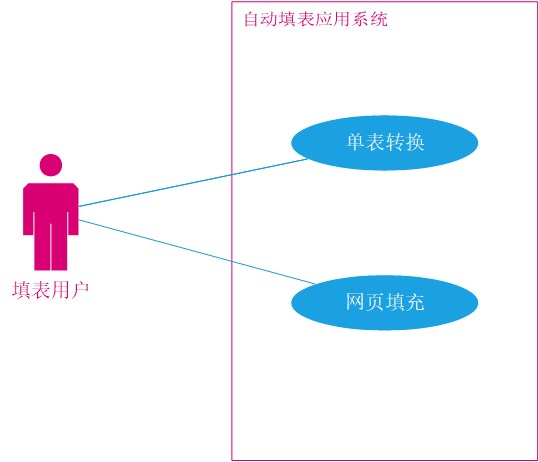
\includegraphics{figures/use_case.jpg}
    \caption{系统用例图,需要填表的用户可以通过与系统交互完成单表转换和网页自动填表两种用例}
    \label{fig:use_case}
\end{figure}

根据面谈的结果,我们将教务员的两种表格转换场景具体定义为了两个系统用例。系统的用例图如图 \ref{fig:use_case} 所示。该系统需要考虑的外界用户只有一类,本文中提到的对该应用进行功能扩展暂需要改动源代码,故不包含在此用例图中。

详细用例描述如图 \ref{fig:use_case_1} 和图 \ref{fig:use_case_2} 所示。

\begin{figure}
    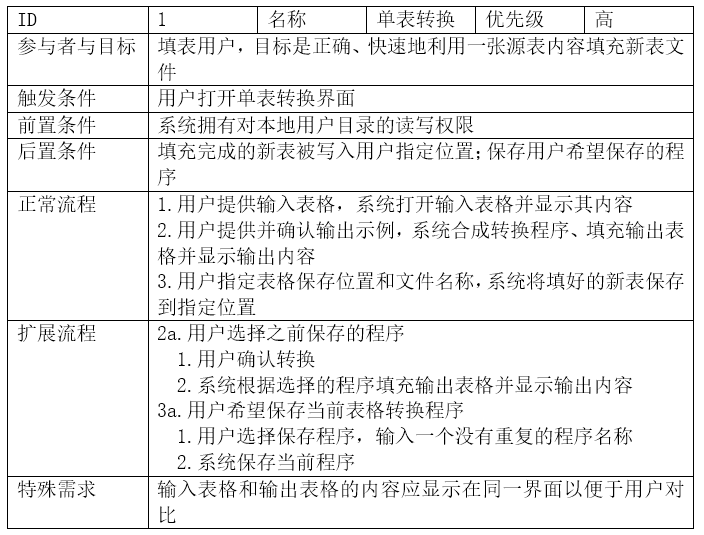
\includegraphics{figures/use_case1.jpg}
    \caption{单表转换用例描述}
    \label{fig:use_case_1}
\end{figure}

\begin{figure}
    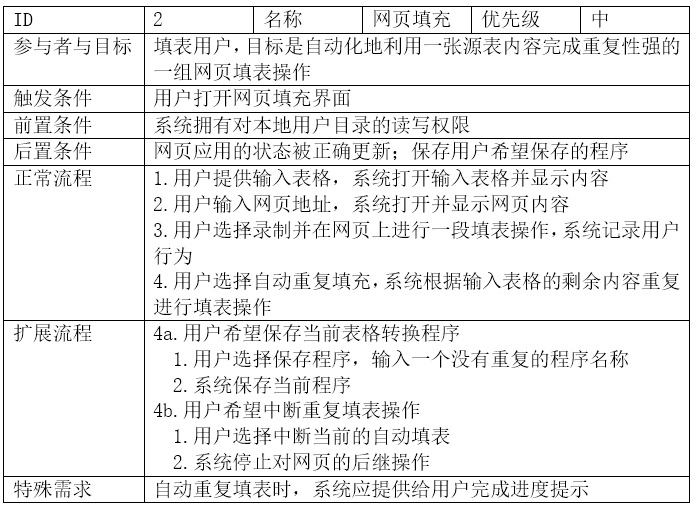
\includegraphics{figures/use_case2.jpg}
    \caption{网页填充用例描述}
    \label{fig:use_case_2}
\end{figure}

\subsubsection{非功能性需求}
$\bullet$可用性需求:
软件可以不经集中培训,立即交付给没有技术背景的普通用户使用。已经有一定办公软件使用经验的用户,应无需查看用户手册即可理解软件的所有功能。软件的表格转换功能可以在离线条件下使用。

$\bullet$安全性需求:
如软件需要用到网络传输和数据库存储,表格内容要在上传到网络前以及在数据库中加密。

$\bullet$可靠性需求:
在用户按照界面指定的要求进行操作后,软件能成功生成所需程序的场合应平均不低于80\%.

\subsection{本章小结}
本章介绍了我们提出的自动填表框架,以及一个以该框架为技术基础,旨在帮助文职人员自动化填表的项目的需求。

\section{第五章~文件模块和网页填表模块的详细设计与实现}
\subsection{文件模块}
该自动填表应用目前支持 csv 格式文件和 docx 格式文件作为源输入文件,csv 格式文件作为单表转换用例的输出文件。

目前,$\mathtt{Table}$在应用中的表示形式是一个字符串类型的二维数组,表格中的空值以长度为0的字符串表示。所有用于处理输入文件的程序最后必须将输入表格转换成该$\mathtt{Table}$格式。

csv 文件逻辑上天然对应了表格,由单元格内容、换行符和逗号分隔符构成。逗号分隔符分隔了一行中任何两个相邻的单元格,行尾是换行符。用于读取 csv 文件的代码如图 \ref{fig:csv} 所示。如需保存 csv 格式的文件,只需进行相反顺序的操作。
\begin{figure}
  \begin{lstlisting}[style=htmlcssjs]
const readCSV = (file, content) => {
  let fileContent;
  if (content !== undefined) {
    fileContent = content;
  } else {
    const buffer = fs.readFileSync(file);
    if (chardet.detect(buffer) === 'UTF-8') {
      fileContent = iconv.decode(buffer, 'utf8');
    } else {
      fileContent = iconv.decode(buffer, ANSI);
    }
  }
  let columnCount = 1;
  let commaCount = 0;
  let columnCountOver = false;
  for (let i = 0; i < fileContent.length; i += 1) {
    if (fileContent.charAt(i) === ',') {
      commaCount += 1;
      if (!columnCountOver) {
        columnCount += 1;
      }
    } else if (fileContent.charAt(i) === '\n' || fileContent.charAt(i) === '\r') {
      if (columnCountOver === false) {
        columnCountOver = true;
      }
    }
  }
  const rowCount = commaCount / (columnCount - 1);
  const table = new Array(rowCount);
  for (let i = 0; i < rowCount; i += 1) {
    table[i] = new Array(columnCount);
  }
  const cells = fileContent.split(/(?:,|\r\n|\r|\n)/);
  for (let i = 0; i < rowCount; i += 1) {
    for (let j = 0; j < columnCount; j += 1) {
      table[i][j] = cells[(i * columnCount) + j];
    }
  }
  return JSON.stringify(table);
};
\end{lstlisting}
    \caption{csv文件读取代码}
    \label{fig:csv}
\end{figure}

docx 文件格式是一种可解压的文件格式,打包了一组 XML 文档,这些文档分别描述 docx 文档的内容、格式和其它元数据。其中,document.xml 文件包含了文档的实际内容,其中的表格部分以 row major order 的顺序记录。当出现合并类型的单元格时,在 document.xml 中实际仍记录的是多个单元格。读取 docx 文件的代码如图 \ref{fig:docx} 所示,解压 docx 后利用正则表达式对 document.xml 中的表格元素进行抽取。\\

\begin{figure}
    \begin{lstlisting}[style=htmlcssjs]
/**
 * Extract tables from a docx to separate CSVs.
 * @constructor
 * @param {string} docxPath - The path of the docx file
 * @return {Array<string>} CSVs - The csv-style contents of each individual table
 * Note that in the result csv each row may not have the same number of columns
 */
function docxToCSV(docxPath) {
  const docx = new AdmZip(docxPath);
  const documentEntry = docx.getEntries().find((entry) => {
    return (entry.name === 'document.xml');
  });
  const document = docx.readAsText(documentEntry);
  const tables = document.match(/<w:tbl[^>]*>(.*?)<\/w:tbl>/g).map((rawXML) => {
    let resultContent = '';
    const rows = rawXML.match(/<w:tr[^>]*>(.*?)<\/w:tr>/g);
    for (let rIndex = 0; rIndex < rows.length; rIndex += 1) {
      const columns = rows[rIndex].match(/<w:tc[^>]*>(.*?)<\/w:tc>/g);
      for (let cIndex = 0; cIndex < columns.length; cIndex += 1) {
        // concat every <w:t> element (blank string if find none)
        const texts = columns[cIndex].match(/<w:t>(.*?)<\/w:t>/g);
        if (texts !== null) {
          for (let tIndex = 0; tIndex < texts.length; tIndex += 1) {
            resultContent += texts[tIndex].replace(/<(\/)?w:t>/g, '');
          }
        }
        if (cIndex !== columns.length - 1) {
          resultContent += ',';
        }
      }
      resultContent += newline;
    }
    return resultContent;
  });
  return tables;
}
    \end{lstlisting}
    \caption{docx文件读取代码}
    \label{fig:docx}
\end{figure}

\subsection{网页填表模块}
鉴于我们没有办法获得网页应用的源码和服务器端,我们采用了纯基于浏览器端的网页录制重放技术。只基于客户端的录制重放技术通常会受到来自服务器端非确定性因素的影响,例如当网页中的内容是由日期、session 信息、第三方服务的调用结果等动态生成的时候,软件行为容易无法完美复现。但对于我们填表的应用场景,表单元素的内容一般不会受到上述因素的影响,相对较为固定,因此这并不是个大问题。由于目前尚不存在成熟的可定制的浏览器端网页录制重放工具,我们参考了 Mickens 等人的工作\cite{mickens10},手动实现了一个通过将网页运行在 Electron 的 webview 中,并在 webview 中运行预加载的 JavaScript 程序来达到效果的录制重放工具。

网页通常是由 HTML 语言编写的树状结构的文档,而 DOM (Document Object Model),又叫文档对象模型,定义了如何通过其它编程语言如 JavaScript 来与 HTML 文档中的内容互动。DOM 定义了网页上可能发生的事件类型和监听它们的接口,网页应用开发者通过调用这些接口,监听具体 DOM 事件来执行相应程序,实现应用逻辑。因此,用户在与一个网页应用进行交互时,实际是具体通过和页面上监听交互事件的元素之间进行交互实现的,如界面上的按钮元素监听鼠标的点击事件、选择框监听选项变更事件、文本框监听键盘输入事件等。用户对这些元素执行相对应的点击、变更选项、输入文字等操作,便会触发这些事件的产生,使对应的 JavaScript 事件处理函数被执行。由于 JavaScript 单线程、函数的执行具有原子性的特征,记录程序的行为不需要具体到代码行的执行顺序,只需记录事件发生的序列和事件的值即可在将来复现页面上的行为。

\begin{figure}
    \centering
    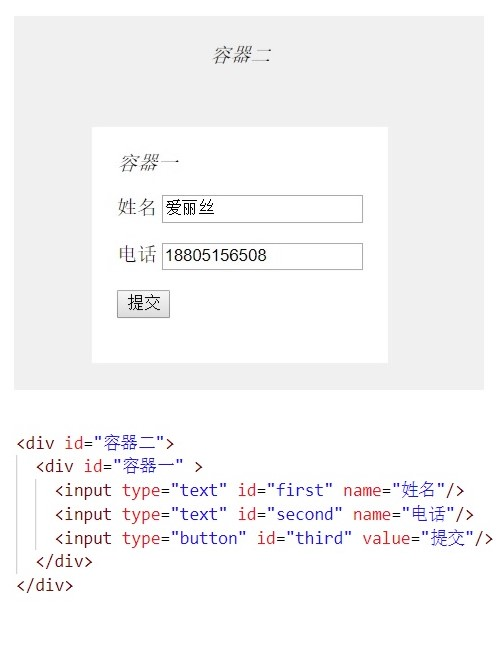
\includegraphics{figures/dom_case.jpg}
    \caption{一个示例的 Web 页面和对应的 HTML 代码。考虑提交按钮,其在 DOM 树中的直接父节点是容器一,再上一级的祖先节点是容器二。容器一和容器二都能监听到提交按钮上发生的事件}
    \label{fig:dom_case}
\end{figure}

为了实现在对页面上内容提前未知的情况下监听特定类型元素上特定事件值,我们利用了 DOM 定义的捕获-目标-冒泡3阶段模型,在一个特殊的位置进行监听。每当一个由 DOM 定义的事件发生时,该事件会首先从根节点出发,沿着父子关系的路径到达事件目标,此过程为捕获阶段。之后,事件目标自己的事件处理函数被触发,这是目标阶段。事件目标自身的处理函数执行结束后,事件再重新从事件目标出发,沿着捕获阶段的反方向传递到根节点,这一过程为冒泡阶段。在3个阶段中,所有涉及到的节点都可以通过 addEventListener() 方法来设置针对特定类型、特定阶段事件的处理函数,并可以通过 Event.target 获得事件目标节点的引用,继而获得目标节点的信息。以图 \ref{fig:dom_case} 为例,如果提交按钮上发生 click 事件,则在捕获阶段中,该事件会从容器二节点开始向下传递(假设容器二节点没有父节点),经过容器一,最后到达提交按钮。在提交按钮已经完成响应后,该事件又会反向经过容器一传递回容器二。 对于在浏览器中运行的网页,最高的根节点是代表当前窗口的 window 节点,即任何网页上的 DOM 事件在传递的过程中一定会经过 window 节点,这一性质为我们无视网页内容的事件监听提供了可能。在录制用户的一段交互行为时,我们只需通过查看 Event.target 的 XPath 和当前值信息,即可知道用户对什么表单元素填了什么值。

DOM 定义的输入元素和事件类型种类众多,我们出于工作量和实际应用场景的考虑,只选择了 
button, select, text 三种元素。由于用户可能会由于填错等原因修改已经填过的值,我们假设用户第一次操作每一个元素的顺序是实际正确的填表顺序,我们记录了这样的顺序,并以结束录制时这些元素上的当前值作为实际填表的值。对于button 类元素,第一次操作是指第一次 click 事件发生;对于 select 类元素,操作是指第一次 change 事件发生;对于 text 类元素,操作是指第一次 focus 事件发生。我们选择的这组事件只是可以用来判断用户进行操作的各种组合中的一种,实际可以根据用户的使用习惯进行调整。我们通过设置 webview 的 preload attribute,在网页内容加载完成前执行我们的特定脚本,为 window 对象添加针对上述类型事件的监听,以 XPath 的形式保存被操作的元素序列。在下次需要填写表格内容时,在页面上执行脚本,修改每个对应元素的值。

为了使我们的重放工具能够在同一 session 里重复填写多次数据,网页内容需要能够在每一组数据填写完成后完成正确的刷新,执行相应的 JavaScript 函数或 HTTP 请求并复原表单。我们观察到这样的刷新行为通常会由用户示例序列中的某按钮点击操作触发,而我们的录制又包括了该按钮的点击,因此刷新通常能够被正确触发。如果网页内容在行为触发后发生了变更,之前的表单元素无法全部找到对应位置,我们会重新载入原网页,填写下一份数据。

在 window 上添加事件处理函数的示例代码如图 \ref{fig:listener} 所示,该函数是用来监听用户对 select 类元素的操作的,其对页面上发生的所有 change 事件在捕获阶段(由 addEventListener() 的最后一个参数决定)进行监听,以防网页应用的实现中阻止了冒泡阶段导致该事件处理函数不被触发。

开始和结束录制的函数如图 \ref{fig:record} 所示,开始录制会对当前记忆的元素进行初始化,等于重新开始录制;结束录制时,查询当前 text 元素中实际填的值(button 和 select 不必查询,是因为其点击操作和选择的值均已在录制阶段记录下来了),完成输入序列的完整构建,并通知 webview 容器外的 Electron 应用代码。

用于重放的函数如图 \ref{fig:replay} 所示,根据新的输入值序列将记忆的 text, select 和 button 元素分别进行赋值、选择和点击的操作。
\begin{figure}
\begin{lstlisting}[style=htmlcssjs]
var inputElementsSequence = [];

var inputElementsIndexMap = new Map(); // key: xpath or id, value: reference to specific elements

var recording = false;

window.addEventListener('change', (e) => {
  if (recording) {
    if (e.target.tagName === 'SELECT') {
      const currentXPath = xpath(e.target);
      if (!inputElementsIndexMap.has(currentXPath)) {
        const newSelectRecord = {
          type: 'select',
          xpath: currentXPath, // the xpath of the select element
          value: e.target.selectedOptions[0].text, // the content of the selected option, not its value attribute
        };
        inputElementsSequence.push(newSelectRecord);
        inputElementsIndexMap.set(currentXPath, newSelectRecord);
      } else {
        inputElementsIndexMap.get(currentXPath).value = e.target.value;
      }
    }
  }
}, true);
\end{lstlisting}
    \caption{事件处理函数示例}
    \label{fig:listener}
\end{figure}

\begin{figure}
\begin{lstlisting}[style=htmlcssjs]
// return the XPath of a dom element, or an iterator for a given xpath expression.
// reference: https://stackoverflow.com/questions/3454526/
// how-to-calculate-the-xpath-position-of-an-element-using-javascript/32623171#32623171
function xpath(el) {
  if (typeof el === 'string') return document.evaluate(el, document, null, 0, null);
  if (!el || el.nodeType != 1) return '';
  if (el.id) return "//*[@id='" + el.id + "']";
  const sames = [].filter.call(el.parentNode.children, function (x) { return x.tagName == el.tagName });
  return xpath(el.parentNode) + '/' + el.tagName.toLowerCase() + (sames.length > 1 ? '['+([].indexOf.call(sames, el) + 1) + ']' : '');
}

function startRecording() {
  inputElementsSequence = [];
  inputElementsIndexMap = new Map();
  recording = true;
}

function stopRecording() {
  // collect current value for all the text elements
  for (let i = 0; i < inputElementsSequence.length; i += 1) {
    const currentElement = inputElementsSequence[i];
    if (currentElement.type === 'text') {
      currentElement.value = xpath(currentElement.xpath).iterateNext().value;
    }
  }
  console.log(inputElementsSequence);
  notifyHostResult();
  recording = false;
}
\end{lstlisting}
    \caption{录制代码}
    \label{fig:record}
\end{figure}

\begin{figure}
\begin{lstlisting}[style=htmlcssjs]
function playSequence(inputSequence) {
  if (typeof inputSequence === 'string') {
    inputSequence = JSON.parse(inputSequence);
  }
  inputSequence.forEach((e) => {
    eNode = xpath(e.xpath).iterateNext();
    switch (e.type) {
      case 'text':
        eNode.value = e.value;
      break;
      case 'select':
        selectByText(eNode, e.value);
      break;
      case 'button':
        eNode.click();
      break;
      default:
    }
  });
}
\end{lstlisting}
    \caption{重放代码}
    \label{fig:replay}
\end{figure}

\subsection{运行示例}
本节通过具体的运行截图和交互描述来介绍苏老师,一位计算机系教务员,是如何通过我们的系统完成她的两个工作中的填表需求的。
\subsubsection{表格转换}
苏老师手上拥有一份某年级所有同学本学期期末成绩的数据表,该文件内容如图 \ref{fig:docx_file} 所示,每个同学每门课都占一行。现在,教务系统需要她上传一张该年级同学必修课的成绩情况,每个同学占一行,姓名后的每一列代表一门具体的必修课。在使用我们的应用之前,苏老师一直采用手动复制粘贴的方式,将每个同学每门课的成绩一个个粘入一张新表里,耗时又容易出错。现在,为了完成这个任务,苏老师打开我们的应用,进入表格转换界面。表格转换界面如图 \ref{fig:ui_1_init} 所示,用户可以在该界面直观地对比源表格式和新表格式。

之后,苏老师选择自己的数据表文件为源文件,并在界面右侧输入一个想要的格式的输出示例,如图 \ref{fig:ui_1_input} 所示。苏老师提供这个输出示例是非常自然的,因为她之前手工处理该任务时的概念就是"贴每个同学的成绩情况"。接下来,苏老师点击填充按钮,稍等片刻后,应用成功生成表格转换程序并填充剩余输出表格,在界面上显示如图 \ref{fig:ui_1_finish} ,正是需要的表格。
\begin{figure}[!htbp]
    \centering
    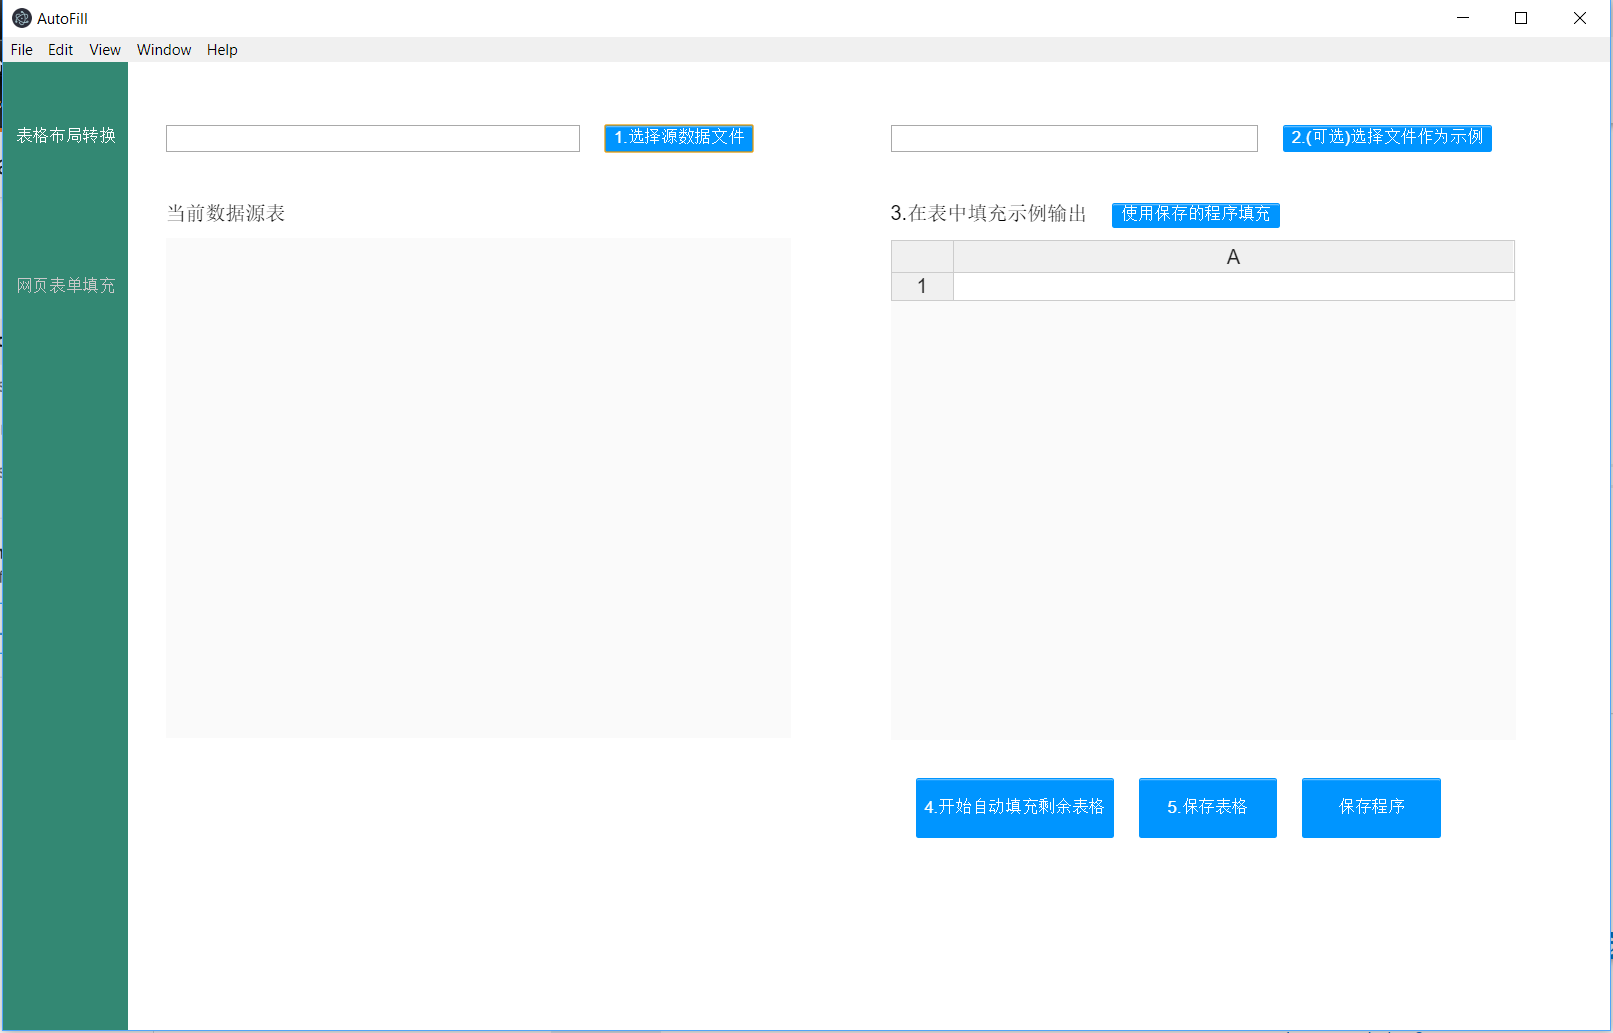
\includegraphics[width=15cm,keepaspectratio]{figures/ui_1_init.png}
    \caption{表格转换起始界面}
    \label{fig:ui_1_init}
\end{figure}
\begin{figure}[!htbp]
    \centering
    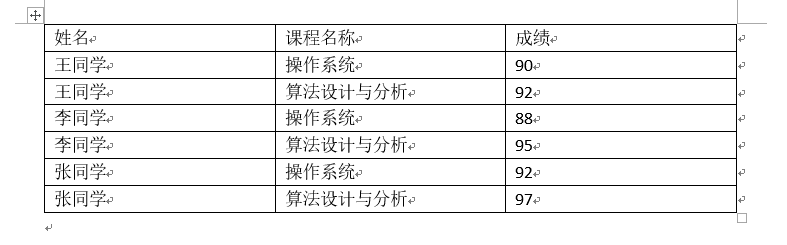
\includegraphics[width=15cm,keepaspectratio]{figures/docx_file.png}
    \caption{表格转换示例源表}
    \label{fig:docx_file}
\end{figure}
\begin{figure}[!htbp]
    \centering
    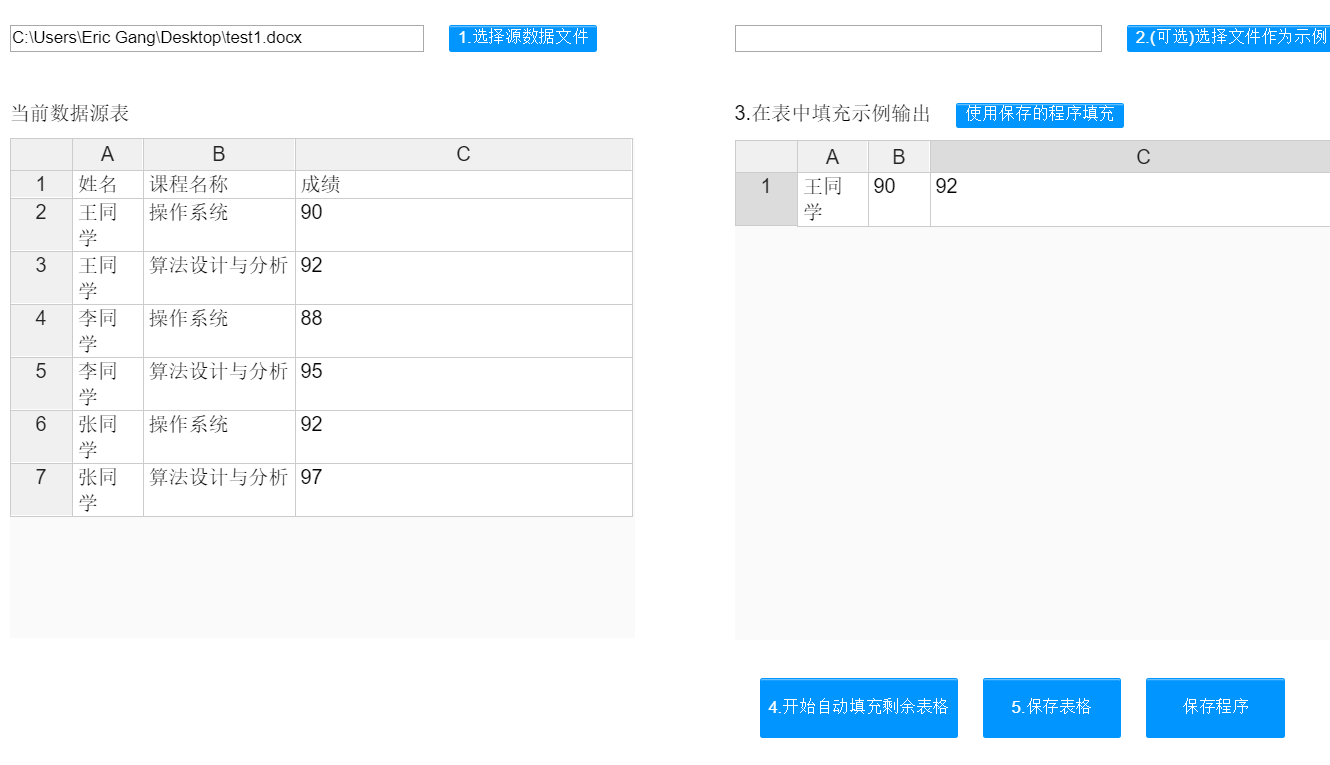
\includegraphics[width=15cm,keepaspectratio]{figures/ui_1_input.png}
    \caption{表格转换示例输入示例}
    \label{fig:ui_1_input}
\end{figure}
\begin{figure}[!htbp]
    \centering
    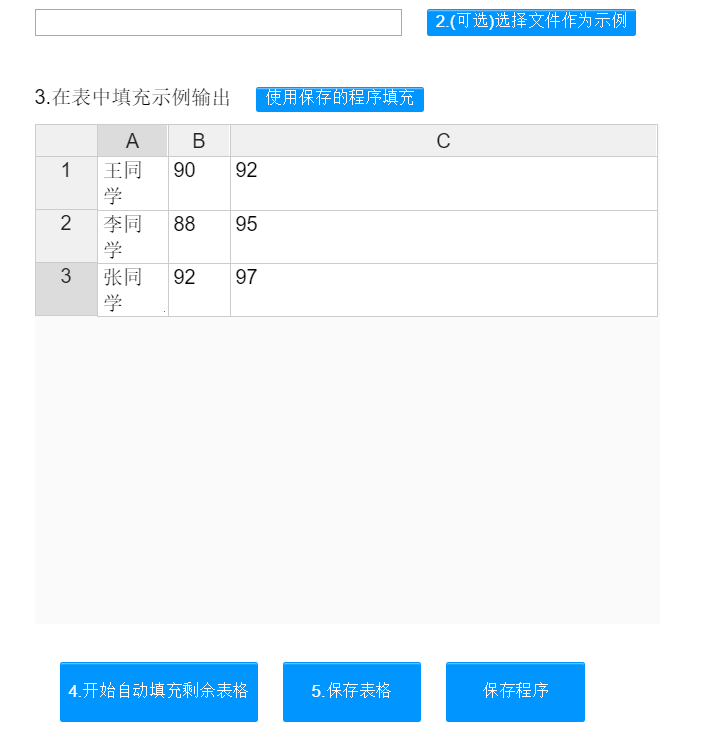
\includegraphics[width=15cm,keepaspectratio]{figures/ui_1_finish.png}
    \caption{表格转换示例填充结果}
    \label{fig:ui_1_finish}
\end{figure}

\subsubsection{网页填充}

每学期开始时,教务员都需要将本学期的课程一门门录入到排课系统中,在使用我们的系统之前,苏老师需要将一张如图 \ref{fig:ui_2_input} 左侧所示的 docx 文件里的课程信息录到类似于该图右侧所示的排课系统里。图 \ref{fig:ui_2_input} 中的表和网页是由苏老师指定打开的。苏老师为了演示她排一门课的操作,点击开始录制,之后开始在页面上进行如下操作:点击课程名称文本框,键入"操作系统",点击任课教师文本框,键入"蒋老师",点击上课人数文本框,键入"80",点击学分数的下拉选择框,选择"4",点击"添加课程"按钮。之后点击结束录制,此时界面如图 \ref{fig:ui_2_record} 所示,页面的课程列表中多的一项是由页面中"添加课程"按钮的事件处理函数生成的。接下来,苏老师点击自动填充,应用开始使用自动化生成的脚本重复在页面上进行相应操作,完成后的结果如图 \ref{fig:ui_2_finish} 所示,每个课程的信息都被正确地输入,每个添加操作都被正确地触发。

\begin{figure}[!htbp]
    \centering
    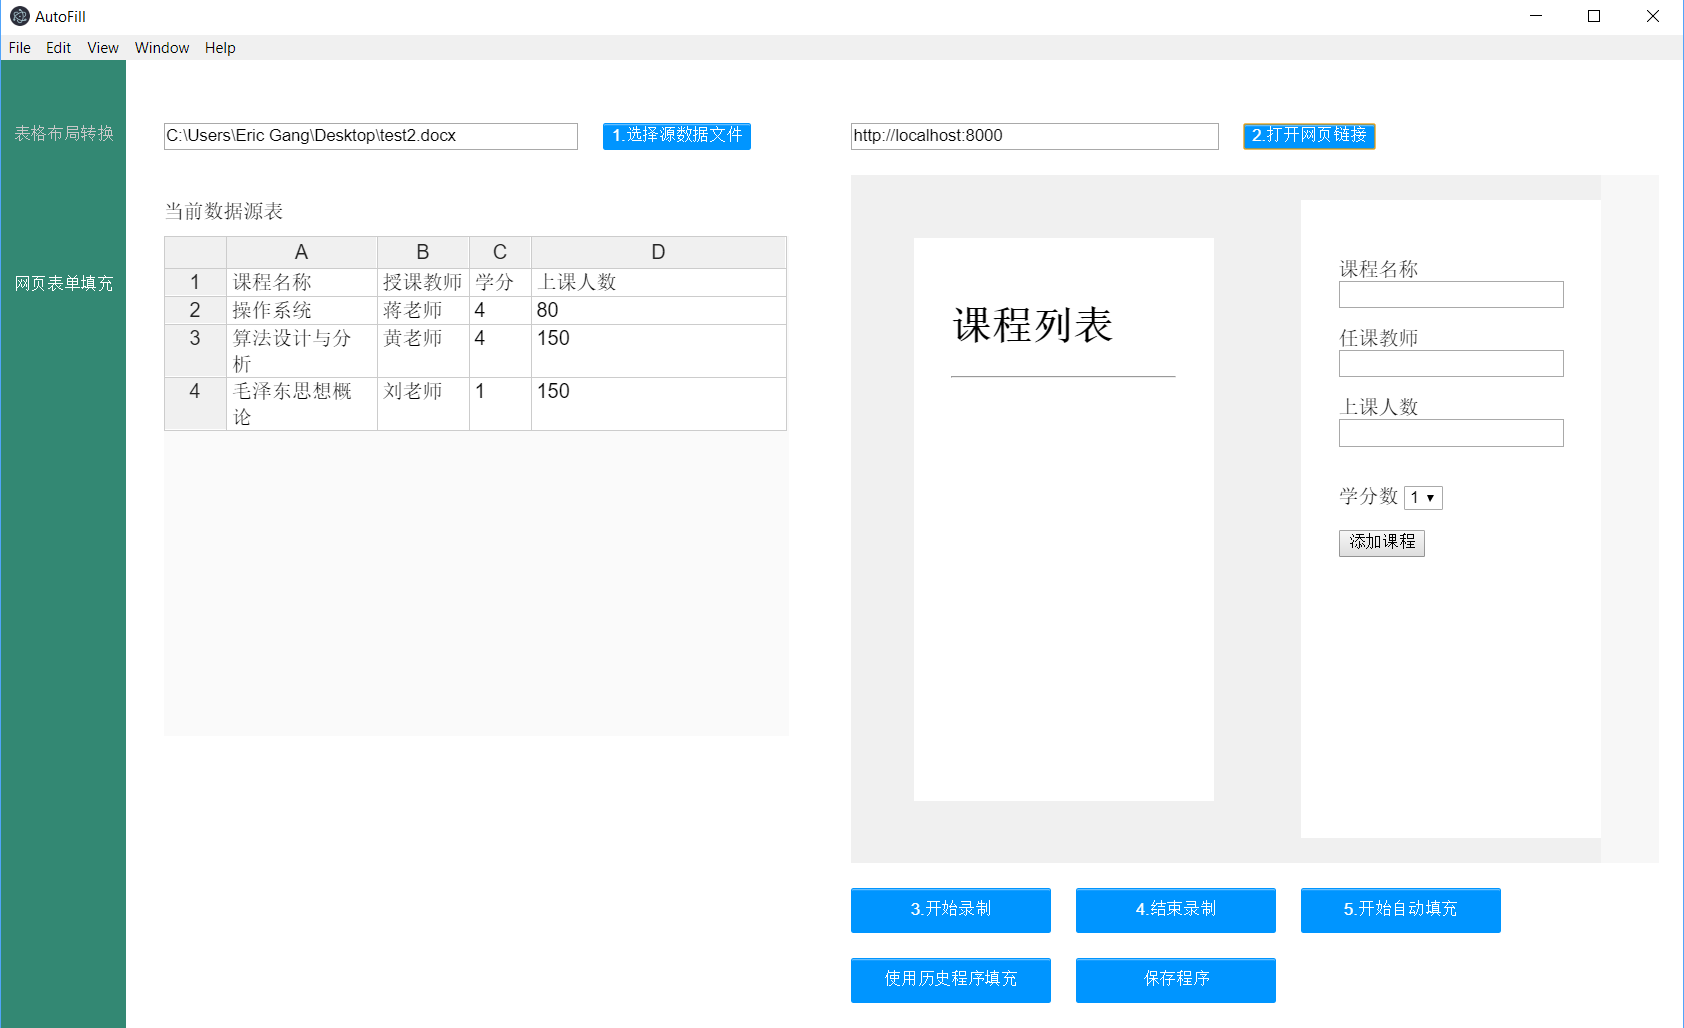
\includegraphics[width=15cm,keepaspectratio]{figures/ui_2_input.png}
    \caption{网页填充示例输入界面}
    \label{fig:ui_2_input}
\end{figure}
\begin{figure}[!htbp]
    \centering
    
\includegraphics[width=15cm,keepaspectratio]{figures/ui_2_record.png}
    \caption{网页填充示例录制操作}
    \label{fig:ui_2_record}
\end{figure}
\begin{figure}[!htbp]
    \centering
    
\includegraphics[width=15cm,keepaspectratio]{figures/ui_2_finish.png}
    \caption{网页填充示例填充结果}
    \label{fig:ui_2_finish}
\end{figure}

\subsection{本章小结}

本章详细描述了在第三章算法和第四章技术框架的基础上,为了满足第四章两个用例的具体需求而实现的文件模块和网页填表模块,并通过两个场景来展现软件所实现了的功能。

\section{第六章~总结与展望}

\subsection{总结}
用户在希望生成脚本自动化自己的填表任务时,往往只希望提供尽可能少的示例,让脚本自动完成重复的其余部分。本份工作展示了一种新的用于表格转换程序语言,其合成算法只需要用户提供部分输出示例,且该方法可以转换已有工作无法转换的任务类型。另外,本份工作描述了一种将此技术用于不同填表应用的框架,并根据实际的用户访谈,设计和实现了一个可以将文档内的表格自动反复填充到网页表单的桌面端应用,可以解决用户长期以来没有被解决的需求,具有广泛的应用前景。

\subsection{展望}
虽然此工作和之前工作相比,用户已经只需要提供更少的信息即部分的输出示例,但覆盖用例范围仍有扩大的空间。目前我们仍然假设用户的一张输出表的所有数据来源为一张表,但用户在填某些新表时可能会需要用到多张不同的旧表的数据,而这些不同旧表的行列的语义可能完全不同,内容又可能有所重叠。如何设计一种适用于多异构数据源的算法,仍然是一个待解决的挑战。

当前自动填充网页表格的实现方式是基于表格元素的 XPath 完全匹配进行识别,即保存的程序会记忆待填元素的 XPath,每遇到一张新表格就往对应的 XPath 上填。这种实现方式部分违背了我们实现跨应用填表的初衷,用户生成的此类程序只能再应用于待填元素的 XPath 没有变更过的同一网页,一旦网页发生影响 XPath 的变更,或用户有跨 web 应用填表的需求如将自己的个人行程信息填到多家不同的旅游网站,就需要重新提供示例、生成相应的转换程序,即使对表格的实际操作是一样的。为不同网页上的表格元素定义相似度的概念,识别出相似的元素序列\cite{wang13},可能能提高该类网页填表程序的普适性。

另外,我们将来计划在此框架上开发更多的扩展,支持更多的输入表格类型和输出类型,如支持基于图像识别的表格录入,支持向移动应用发送生成的表格数据等,来提高该自动填表应用的泛用性。

\newpage
\pagenumbering{Roman}

\bibliographystyle{njubachelor}
\bibliography{ref}

\newpage
\ack

我首先要特别感谢我的导师,模范和挚友:蒋炎岩,是他对电子表格独到的见解提供了该工作的问题雏形。他拥有真正热爱一个专业的人身上的独特品质。能遇到他做为我的研究和毕设导师,从他身上学习做研究的态度和计算机科学相关的各类知识,是我本科经历中最大的荣幸。

我的家人值得特别的感谢。他们一直支持我做任何我想做的事情,几乎从不在我的学业选择上施加压力,正因如此我才能无所顾忌地寻找并找到自己真正感兴趣的研究话题。

我还想额外感谢软件所 SPAR 小组,尤其是程序合成小组里的一些老师和同学,包括但不限于许畅老师,吴嘉荣同学,赵泽林同学,李达同学,石丰民同学,陈劭源同学和凌浩同学。他们中的每一个人都曾在交流中给过我或是新颖的问题视角,或是有趣的备选方案,又或是鼓励我的真诚话语。没有他们的影响,这份工作可能就不会出现。

\newpage
\appendix

\end{document}
